\question Os transdutores de temperatura de um determinado tipo são enviados em lotes de 50. Uma amostra de 60 lotes foi selecionada e o número de transdutores fora das especificações em cada lote foi determinado, resultando nos dados a seguir:
\begin{parts}
    \part Determine as frequências simples e relativas \footnote{Proporção da frequência em relação a amostra.} dos valores de x = número de transdutores fora das especificações em um lote.
    \begin{solution}
        % latex table generated in R 4.3.3 by xtable 1.8-4 package
        % Sun Mar 31 22:05:33 2024
        \begin{table}[H]
            \centering
            \begin{tabular}{rlrr}
                \hline
                   & fora  & Freq        & FreqRel    \\
                \hline
                1  & 0     & 7.00000000  & 0.11666667 \\
                2  & 1     & 12.00000000 & 0.20000000 \\
                3  & 2     & 13.00000000 & 0.21666667 \\
                4  & 3     & 14.00000000 & 0.23333333 \\
                5  & 4     & 6.00000000  & 0.10000000 \\
                6  & 5     & 3.00000000  & 0.05000000 \\
                7  & 6     & 3.00000000  & 0.05000000 \\
                8  & 7     & 1.00000000  & 0.01666667 \\
                9  & 8     & 1.00000000  & 0.01666667 \\
                \hline
                10 & Total & 60.00000000 & 1.00000000 \\
                \hline
            \end{tabular}
        \end{table}

    \end{solution}

    \part Que proporção de lotes na amostra possui no máximo cinco transdutores fora das especificações? Que proporção tem menos de cinco? Que proporção possui no mínimo cinco unidades fora das especificações?
    \begin{solution}
        Para aqueles que possuem no máximo cinco transdutores fora temos aqueles que possuem 0, 1, 2, 3, 4 e 5, logo a proporção é de 0.11666667 + 0.20000000 + 0.21666667 + 0.23333333 + 0.10000000 + 0.05000000 = 0.91666667.

        Para aqueles que possuem menos de cinco transdutores fora temos aqueles que possuem 0, 1, 2, 3 e 4, logo a proporção de 0.11666667 + 0.20000000 + 0.21666667 + 0.23333333 + 0.10000000 = 0.86666667.

        Para aqueles que possuem no mínimo cinco transdutores fora temos aqueles que possuem 5, 6, 7 e 8, logo a proporção de 0.10000000 + 0.05000000 + 0.05000000 + 0.01666667 + 0.01666667 = 0.23333333.
    \end{solution}

    \pagebreak

    \part Faça a representação gráfica dos dados.
    \begin{solution}
        \begin{figure}[H]
            \centering
            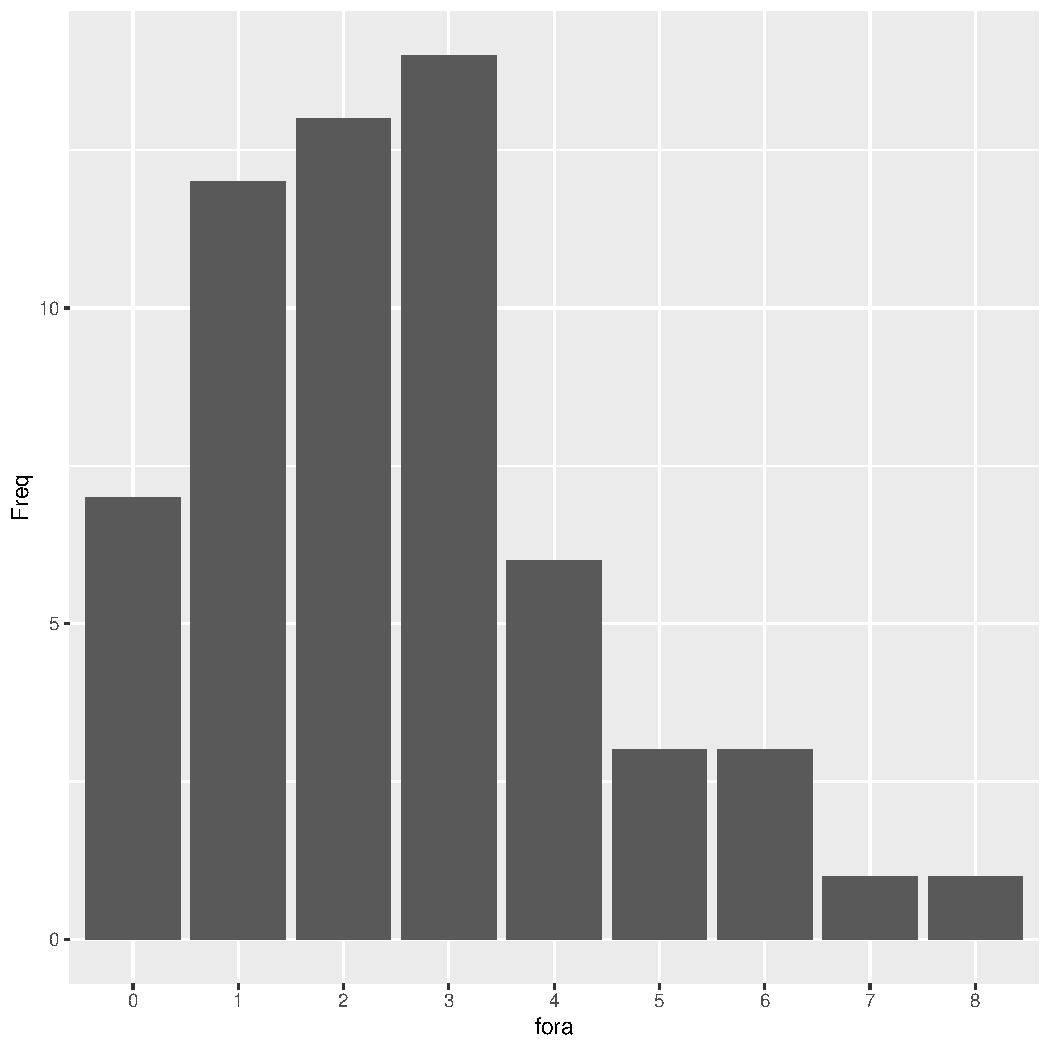
\includegraphics[width=8cm]{./../src/output/03312024_Output_BarNumTransdutores.pdf}
        \end{figure}
    \end{solution}
\end{parts}
